\documentclass[aps,prd
,tightenlines,letterpaper,
%superscriptaddress,
nofootinbib]{revtex4-1}

\usepackage{amssymb,latexsym}
\usepackage{amsmath,amsbsy,bbm}
\usepackage{epsfig,bm,color}
\usepackage{graphicx,comment}
\usepackage[vcentermath]{youngtab}
\usepackage{slashed}
\usepackage{nicefrac}

\unitlength=1mm

\DeclareMathOperator{\st}{str}
\DeclareMathOperator{\tr}{tr}
\DeclareMathOperator{\Erfc}{Erfc}
\DeclareMathOperator{\Erf}{Erf}
\DeclareMathOperator{\Pf}{Pf}
\DeclareMathOperator{\sign}{sign}

\usepackage{dutchcal}
\usepackage{calligra}

\DeclareMathAlphabet{\mathcalligra}{T1}{calligra}{m}{n}
\DeclareFontShape{T1}{calligra}{m}{n}{<->s*[2.2]callig15}{}
\newcommand{\scriptr}{\mathcalligra{r}\,}
\newcommand{\boldscriptr}{\pmb{\mathcalligra{r}}\,}


\begin{document}

\newcommand{\eftnopi}{\mbox{EFT$(\not \! \pi)$}}
\newcommand{\ve}[1]{\ensuremath{\boldsymbol{#1}}}
\newcommand{\ecm}{\ensuremath{E_\text{\tiny cm}}}
\newcommand{\ls}{\ve{L}\cdot\ve{S}}
\newcommand{\ent}{~\widehat{=}~}

\def\a{{\alpha}}
\def\b{{\beta}}
\def\d{{\delta}}
\def\D{{\Delta}}
\def\X{{\Xi}}
\def\e{{\varepsilon}}
\def\g{{\gamma}}
\def\G{{\Gamma}}
\def\k{{\kappa}}
\def\l{{\lambda}}
\def\L{{\Lambda}}
\def\m{{\mu}}
\def\n{{\nu}}
\def\o{{\omega}}
\def\O{{\Omega}}
\def\S{{\Sigma}}
\def\s{{\sigma}}
\def\th{{\theta}}

\def\ol#1{{\overline{#1}}}


\def\Dslash{D\hskip-0.65em /}
\def\Dtslash{\tilde{D} \hskip-0.65em /}

\def\ie{{\it i.e.~}}
\def\wrt{{\it w.r.t.~}}
\def\eg{{\it e.g.~}}
\def\he#1{{{}^#1\text{He}}}
\def\li#1{{{}^#1\text{Li}}}
\def\QCPT{{Q$\chi$PT}}
\def\PQCPT{{PQ$\chi$PT}}
\def\tr{\text{tr}}
\def\str{\text{str}}
\def\diag{\text{diag}}
\def\order{{\mathcal O}}

\def\cF{{\mathcal F}}
\def\cG{{\mathcal G}}
\def\cE{{\mathcal E}}
\def\cS{{\mathcal S}}
\def\cC{{\mathcal C}}
\def\cB{{\mathcal B}}
\def\cT{{\mathcal T}}
\def\cQ{{\mathcal Q}}
\def\cL{{\mathcal L}}
\def\cO{{\mathcal O}}
\def\cA{{\mathcal A}}
\def\cQ{{\mathcal Q}}
\def\cR{{\mathcal R}}
\def\cH{{\mathcal H}}
\def\cW{{\mathcal W}}
\def\cM{{\mathcal M}}
\def\cD{{\mathcal D}}
\def\cZ{{\mathcal Z}}
\def\cN{{\mathcal N}}
\def\cP{{\mathcal P}}
\def\cK{{\mathcal K}}
\def\Qt{{\tilde{Q}}}
\def\Dt{{\tilde{D}}}
\def\St{{\tilde{\Sigma}}}
\def\cBt{{\tilde{\mathcal{B}}}}
\def\cDt{{\tilde{\mathcal{D}}}}
\def\cTt{{\tilde{\mathcal{T}}}}
\def\cMt{{\tilde{\mathcal{M}}}}
\def\At{{\tilde{A}}}
\def\cNt{{\tilde{\mathcal{N}}}}
\def\cOt{{\tilde{\mathcal{O}}}}
\def\cPt{{\tilde{\mathcal{P}}}}
\def\cI{{\mathcal{I}}}
\def\cJ{{\mathcal{J}}}

\def\eqref#1{{(\ref{#1})}}

\newcommand{\duo}[2]{\ensuremath{\arraycolsep=4pt\def\arraystretch{2}
	\begin{array}{c}
	#1\\
	#2
	\end{array}}
}

\newenvironment{ecce}[1][Ecce]{\begin{trivlist}\scriptsize\color{blue}
\item[\hskip \labelsep {\bfseries{\color{red} #1}}]}{\end{trivlist}}

\newenvironment{definition}[1][Definition]{\begin{trivlist}
\item[\hskip \labelsep {\textrm{\bfseries#1}}]}{\end{trivlist}}

 
\title{
List of calculations might be useful to understand the problem
} 

\begin{abstract}
What kind of calculations should be done to understand the limits of \eftnopi at LO? 
We have three degrees of freedom (not completely unrelated) $C_{2b}$, $D_{3b}$, and the cut-off $\lambda$
\end{abstract}

\pacs{}
 
\maketitle


\section{Scales of the system and anzatz}
In all this small vademequm I will define as $a$, $b$, $c$, .. identical \textit{bosons} or different fermions with \textit{symmetric} spacial wave functions, while I will relate identical \textit{fermions} using the same letter (I.E. $aa$, $bb$, ..)
The independent scales of our problem are essentially two: $a_0=a_0(ab)=a_0(ac)=a_0(bc)=..$ and the 3-body binding energy $B_{3b}$.
The cut-off, we assume, should go to infinity, but the only reference scale for it is the 2-body scattering length (we assume the effective range $r_0=0$), therefore $\lambda \gg 1/a_{0}$ is enough.

\begin{figure}[h] 
\centering 
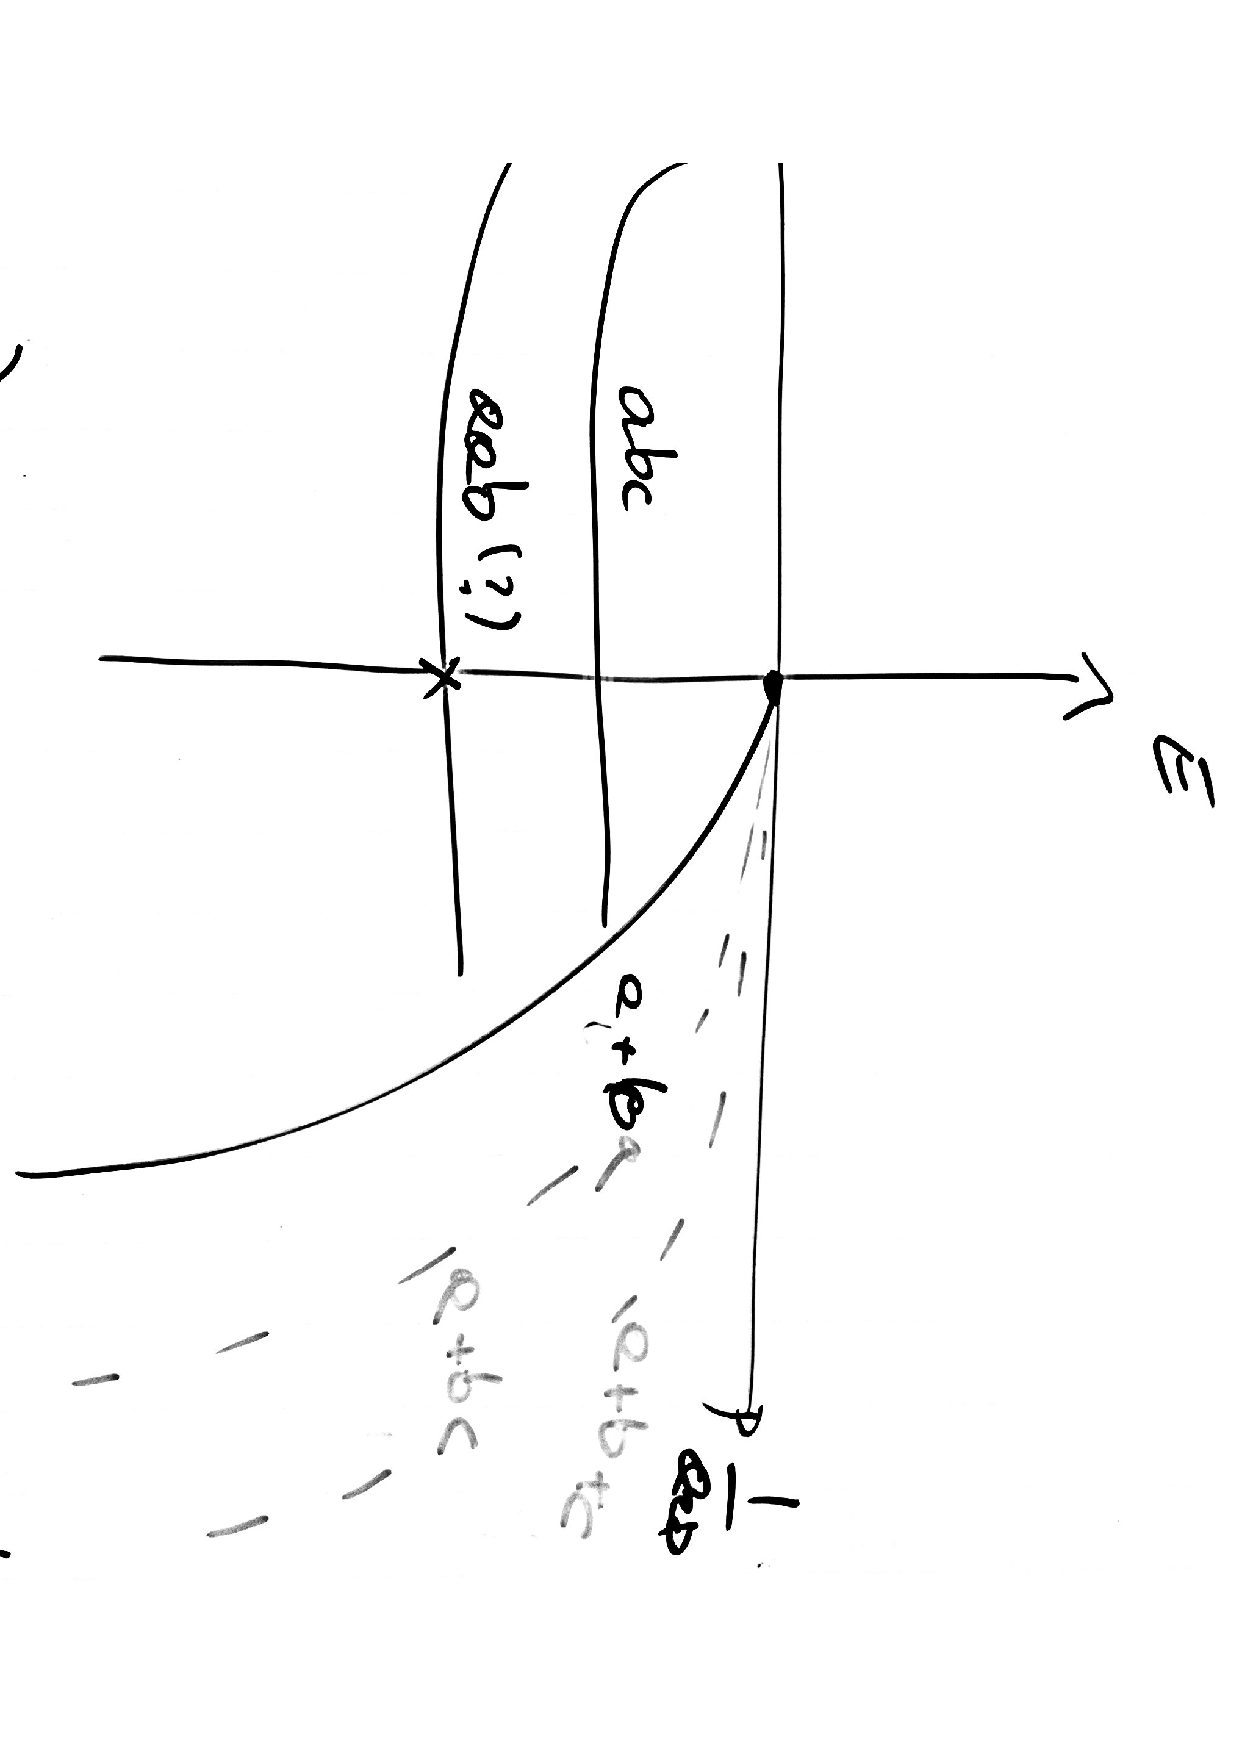
\includegraphics[width=0.5\textwidth,angle=90]{./efimovaab.pdf} 
\label{fig:ef_plot}
\caption{} 
\end{figure} 

Assuming that we can draw a plot similar to the Efimov plot for bosonic systems $abc$ (the usual one) also for $aab..z$ systems Fig. \ref{fig:ef_plot}, the best place to look for L=1 3-body bound states is close to the $ab$ unitary limit.
In this case the 2-body system is very extended, relatively to the physical systems, therefore each cut-off we take will be very large.
E.g. if we take a scattering length of -100 fm, the minimum cut-off scale of the theory will be around 2 MeV.


\section{Technical point of the calculations}

What we want to show is in which system \eftnopi is able, under certain conditions, to produce bound states and possibly resonances.
To do this we should choose the most "favorable" situation to create bound states, which, according to Fig. \ref{fig:ef_plot} is with $a_0\rightarrow\infty$.
To make life easy we should chose a shallowly bound 2-body system ($a_0\sim-10$ to $-100$ fm) to make our codes happy and less unstable.
The 3-body LEC is not relevant since in the systems $aab..z$ it will just shift the threshold energy, but, in the unitary limit, it will not make a possible bound state disappear.
For simplicity sake we want to have one and just one $abc$ bound state, possibly close to threshold so we can easily identify further $aab..z$ bindings and we are not in the Boromean region ($aabc$ bound but $abc$ is not).

But how to proceed in the best systematic and rational way is a still open query that require further investigations. It follows my suggestion.

\subsection{Step 0)}
Just calculate $^6$Li and $^4$He+$^2$H and show that pionless thory do not bind this systems for $\lambda=2,4,6,8$ fm$^{-1}$.
This will show the importance of this paper.

\subsection{Step A)}
Probably first we want to calculate systems with fixed $a_0$ and $E_3b$ for multiple cut-off:

$\lambda = [1/2, 1,2,5,10,20,50]\, 1/a_0$

Fit: $B_{ab}=1$ MeV, $B_{abc}=2$ MeV

Systems: $aab,\, aabc,\, aabcd,\, aabcde,\, aacc,\, aabbc,\, aabbcd$

Which correspond to the nuclear systems: $^3$n, $^4$H, $^5$He, $^6_\Lambda$He, $^4$n, $^5$H, $^6$He.

\textit{what we expect:}  the energy of those system approach the S-wave core energies.

Later we can also investigate: $aabbcc$, $aabbccd$ and $aabbccdd$.

\begin{center}
\begin{tabular}{ l ccccccc }
 S-core: & ab &abc & abcd & abcde&&& \\
 P-wave: & aab & aabc & aabcd & aabcde & aacc & aabbc & aabbcd \\ 
 Expected enrgy: & ab & abc & abcd & abcde & 2$\times$ac & abc+ab & abcd+ab\\
\end{tabular}
\end{center}

\subsection{Step B)}

To \textbf{not} find a boundstate is cool, but we want to show what happen if we \textit{manufact} a P-wave bound state and show that it forcefully disappear when $\lambda\rightarrow\infty$.

I suggest to fit $C_{2b}$ to reproduce $aab=ab+1$MeV and to calculate $ab$.

We expect to see $B(ab)\xrightarrow[]{\lambda\rightarrow\infty}\infty$.

The same should happen if we fit $aabb$ and we calculate $ab$.

We need to do it for a set of cut-offs: $\lambda = [1/2, 1,2,5,10,20,50]\, 1/a_0$


\subsection{Step C)}

what happen if we change the three body instead of the two body? we can fit $D_{3b}$ on $aabc=abc+1$ MeV and see that $B(abc)\xrightarrow[]{\lambda\rightarrow\infty}\infty$.

Same as before.

\begin{figure}
\[\arraycolsep=4pt\def\arraystretch{4}
\begin{array}{l|lllll}
AB\ldots Z &  (AB\ldots Z)A & (AB\ldots Z_\text{even})^n & (AB\ldots Z_\text{odd})^n & & \\
\duo{\yng(2) }{ {}^2n, np} &
\duo{\yng(2,1)}{ {}^3\text{n}, \left({}^3\text{He}\right)^3} &
\duo{\yng(2,2)}{ {}^4n} &
\duo{\yng(1,1)}{{}^2n(S=1)} &
\duo{\yng(3,2)}{{}^5\text{H(e)}} & 
\duo{\yng(4,2)}{{}^6\text{Li}} \\
\duo{\yng(3)}{ {}^3\text{H(e)}} &
\duo{\yng(3,1)}{{}^4\text{H}} &
\duo{\yng(4,4)}{{}^8\text{Be}} &
\duo{\yng(3,3)}{{}^6\text{Li}} &
\yng(4,3) &
\yng(6,2) \\
\duo{\yng(4)}{{}^4\text{He}} & 
\duo{\yng(4,1)}{{}^5\text{H(e)}} & 
\duo{\yng(4,4,4)}{{}^{12}\text{C}} & 
\yng(3,3,3) &  &  \\ \hline
\yng(5) & 
\yng(5,1) & &  &  &  \\
\yng(6) & 
\yng(6,1) & &  &  &  \\
\yng(7) & \yng(7,1) & &  &  &  \\
\yng(8) & \yng(8,1) & &  &  &  \\\hline
\begin{minipage}[c]{.15\textwidth}
generalization of the universal ratio $\lim\limits_{n\to\infty}\frac{B_n}{B_{n-1}}$ to
$\frac{B_n(A)}{B_{n}(A+1)}\stackrel{?}{=}f(A)$
\end{minipage} &
\begin{minipage}[c]{.15\textwidth} odd-odd (imbalanced)\\effect of additional bosons to which the $2^\text{\tiny nd}$ fermion can bind; no additional exchange effect from one system size to the other.
\end{minipage} &
\begin{minipage}[c]{.15\textwidth} even-even (balanced)\\exchange effects in combination
with increasing number of cross-fragmentinteractions.
\end{minipage} &
\begin{minipage}[c]{.15\textwidth}odd-odd (balanced) same as even-even (triplet vs. doublet)
\end{minipage} &
\begin{minipage}[c]{.15\textwidth}
\end{minipage} &
\begin{minipage}[c]{.15\textwidth}
\end{minipage} \\
\end{array}
\]\caption{\small Classification of $A$-body systems according to particle number and
accessible internal states.}
\end{figure}


\newpage
\bibliographystyle{unsrt}
\bibliography{Thebibliography.bib}

\end{document}